\chapter{Mathematical Definitions for Signals and Systems}

\section{Defining Signals}
Because a signal is fundamentally a function, the conventions of defining a signal closely follow the conventions of defining a function.
For example, suppose we would like to define an audio signal as a function of time that returns the soundwave air pressure of some specific point, then we can simply define this function declaratively as:
\[
    \forall t \in {\rm Time}, s(t) = \sin(440 \times 2\pi t)
\]
which states that the air pressure of our sound signal is a sinusoidal function with respect to time.

On the other hand, we may also define our function imperatively when programming the signal, which would result in the portrayal of abbove function using code:
\begin{verbatim}
import numpy as np
signal = lambda t: np.sin(440 * 2 * np.pi * t)
\end{verbatim}
You will be frequently using imperative definitions in lab assignments, and declarative definitions when working with the mathematical representation of signal in homework assignments or exams.

\section{Defining Systems}
\subsection{A Review of Systems}
Remember that we define systems as functions that map an input signal space (a space of all possible input signals) onto an output signal space.
Therefore, systems are functions whose domains and ranges can be expressed in: $S: [D \rightarrow R] \rightarrow [D' \rightarrow R']$.
Alternatively, we can describe a system $S$ with the graph of its corresponding function:
\[
    \{(x, S(x)) | x \in [D \rightarrow R]\}
\]
Such graph fundamentally describes every possible input-output signal pair, which directly depicts the system's behavior upon any provided input.
Therefore, we also address the graph of a system's function $S$ as its behavior.

What about using a table instead of a graph?
Unfortunately, there is usually too many input signals to consider for a system.
The construction of tables assume a finite input domain and finite output domain, and needs to exhaustively list all input-output correspondences.
However, systems very often encounter an infinite input domain (which means there can be infinite possible inputs), if not an extremely large input domain (eg., the set of all possible $1920\times1080$ pictures).
Therefore, tables are less practical choices for mathematical representations of system behavior than sets are.

\subsection{Systems and Its Memories}
A system is \textbf{memoryless} when it only depends on the current input state. We call such systems ``memoryless'' by the fact that it only depends on the present input, but neither past input nor information regarding timestep.
\begin{ln-define}{Memoryless Systems}{}
    To ensure that a system $F: [\mathbb{R} \rightarrow Y] \rightarrow [\mathbb{R} \rightarrow Y]$ is memoryless, we require that there exists a function $f: Y \rightarrow Y$ such that:
    \[
        \forall t \in \mathbb{R}, x \in [\mathbb{R} \rightarrow Y], (F(x))(t) = f(x(t))
    \]
    such that the system $F$ can be portrayed as a function that solely depends on the current input $x(t)$.
\end{ln-define}

On that note, a system with memory would be any system whose expression $(F(x))(t)$ relies on information outside of $x(t)$.
Let us refine our understanding with a couple of examples below:
\begin{ln-example}{An Example of Memoryless System}{}
    Suppose our system $S$ receives an input signal $x$ and outputs signal $y$ such that:
    \[
        \forall t \in \mathbb{R}, y(t) = {x(t)}^2
    \]
    In such case, we can model the system's relation solely upon the value of $x(t)$, so the system is memoryless.
\end{ln-example}

\begin{ln-example}{An Example of System with Memory}{}
    Suppose our system $S$ receives an input signal $x$ and outputs signal $y$ such that:
    \[
        \forall t \in \mathbb{R}, y(t) = \sum_{t'=0}^{t-1} {(0.99)}^{t - t'} x(t')
    \]
    Becuase this system's relation depends on information outside of current input, such as past input signals and timestep information, this system has and requires memory.
\end{ln-example}

\subsection{Using Difference and Differential Equations}
Systems can also be defined using equations that model the inner dynamics of the system.
For continuous signals, such equations are differential equations, which are equations that describe the rate of change of a variable as an expression of that variable.
These equations will be frequently encountered at the end of MATH 1B, as well as some aspects of this course.
\[
    \dv{y(t)}{t} = x(t) + \lambda y(t)
\]

Meanwhile, discrete signals use difference equations because differential equations are not fitting for non-continuous functions like discrete-time functions.
Difference equations are equations that relate the output signal with the input signal; essentially, it is the expression of the system function.
For example:
\[
    y(n) = \frac{x(n) + x(n - 1)}{2}
\]

\subsection{Block Diagrams as Schematics}
A block diagram is a visual summary of system using blocks to represent the components of a complicated larger system.
Usually, block diagrams are presented on design blueprints and research papers to help readers visually summarize the schematics of a large system.
Let's use the following block diagram, which protrays the system:
\[
    \forall t \in \mathbb{R}, S_1(x)(t) = y_1(t) = x(t)^2 + 2x(t) + \frac{1}{x(t)}
\]
as an example:

\begin{center}
    \begin{figure}[h]
        \centering
        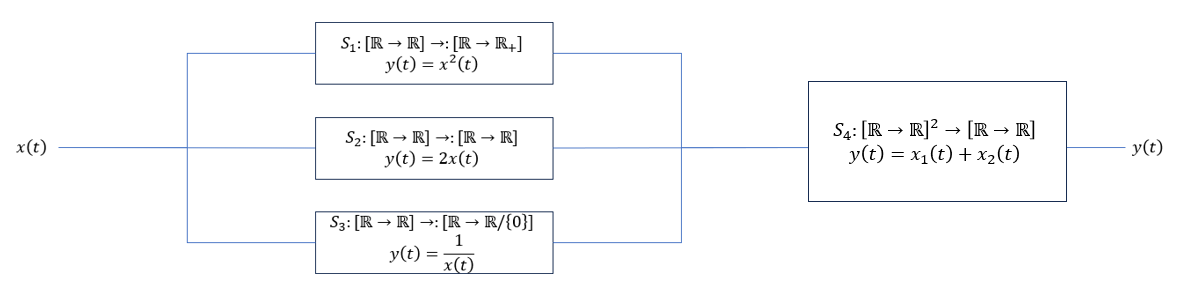
\includegraphics[width=0.9\textwidth]{figs/ln06/example_block_diagram.png}
        \caption{Example block diagram of the above memoryless system.}
    \end{figure}
\end{center}

In a block diagram, each block resembles one smaller component of the system (which can also be a system) that maps the input signal into some intermediate form (which can also be an output signal).
Ideally, each block only resembles one function.
Then, throughout the block diagram, the outputs of each block become the input of its connected blocks, flowing from left to right.
It provides us a graphical comprehension of the system we deal with.

Occassionally, our systems would require memory, which means that we may rely on information about the past input signals.
For example, such system:
\[
    \forall t \in \mathbb{R}, S_2(x)(t) = y_2(t) = y_2(t - 1) + \frac{1}{x(t)}
\]
The connection from a previous output state into a current output state's computation is known as a \textbf{feedback}.
This name is intuitive in the sense that whenever a feedback occurs, it is that a previous output state feeds back to another current output state (and this can be either additive or subtractive, sometimes even multiplicative).
Let us see how a block diagram would work with this information:
\begin{center}
    \begin{figure}[h]
        \centering
        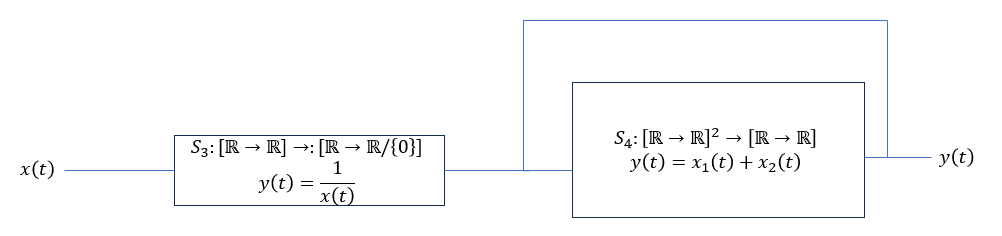
\includegraphics[width=0.9\textwidth]{figs/ln06/example_feedback_block.png}
        \caption{Example block diagram of the above memory system.}
    \end{figure}
\end{center}

In a block diagram, feedbacks are portrayed by connections between the output state per se and the associated computing blocks.
In the above diagram, the output signal's output value, $y(t)$, will be fed into the system's adder block in the next timestep $t+1$ to achieve the recrusive formula above.
